\chapter{Package \texttt{bank}}

This is a module that generates a template bank to search for
inspiralling and merging binaries consisting of neutron stars
and/or black holes. Template placement is based on the geometrical
formalism \cite{Owen:96,OwenAndSathyaprakash:99}.  A user
calls either \texttt{LALInspiralCreateCoarseBank,}
to create a coarse bank, or \texttt{LALInspiralCreateFineBank,}
to create a fine bank, at specified minimal matches.
\texttt{LALInspiralCreateCoarseBank} first chooses templates
along the $\eta=1/4$ curve and then systematically lays a
rectangular grid in the $\tau_0$-$\tau_2$ plane, or $\tau_0$-$\tau_3$
plane depending on user's choice.

If the metric on a (two-dimensional) signal manifold characterised
by parameters $(x_0,x_1)$ is $g_{ij}$ then the spacing between templates
is given by
\begin{equation}
   dx_0 = \sqrt{ \frac{2(1 -MM)}{g_{00}} },\ \
   dx_1 = \sqrt{ \frac{2(1 -MM)}{g_{11}} }.
\end{equation}

\section{Template Placement for Binary Inspiral Searches}
{\it Template placement} is a problem of populating the binary
parameter space (masses, spins, etc.) with as small a number of
templates as possible, subject to the constraint that every signal
that lies within the space has an overlap greater
than or equal to a certain {\it minimal match} with at least one template in
the grid. Past studies \cite {Sathyaprakash and Dhurandhar 1991, Sathyaprakash 1994, OwenAndSathyaprakash:99}
have shown that this is most easily achieved by using the space of
{\it chirp-times} to lay templates rather than the space of component masses.

\begin{figure}[h]
\centering {
\noindent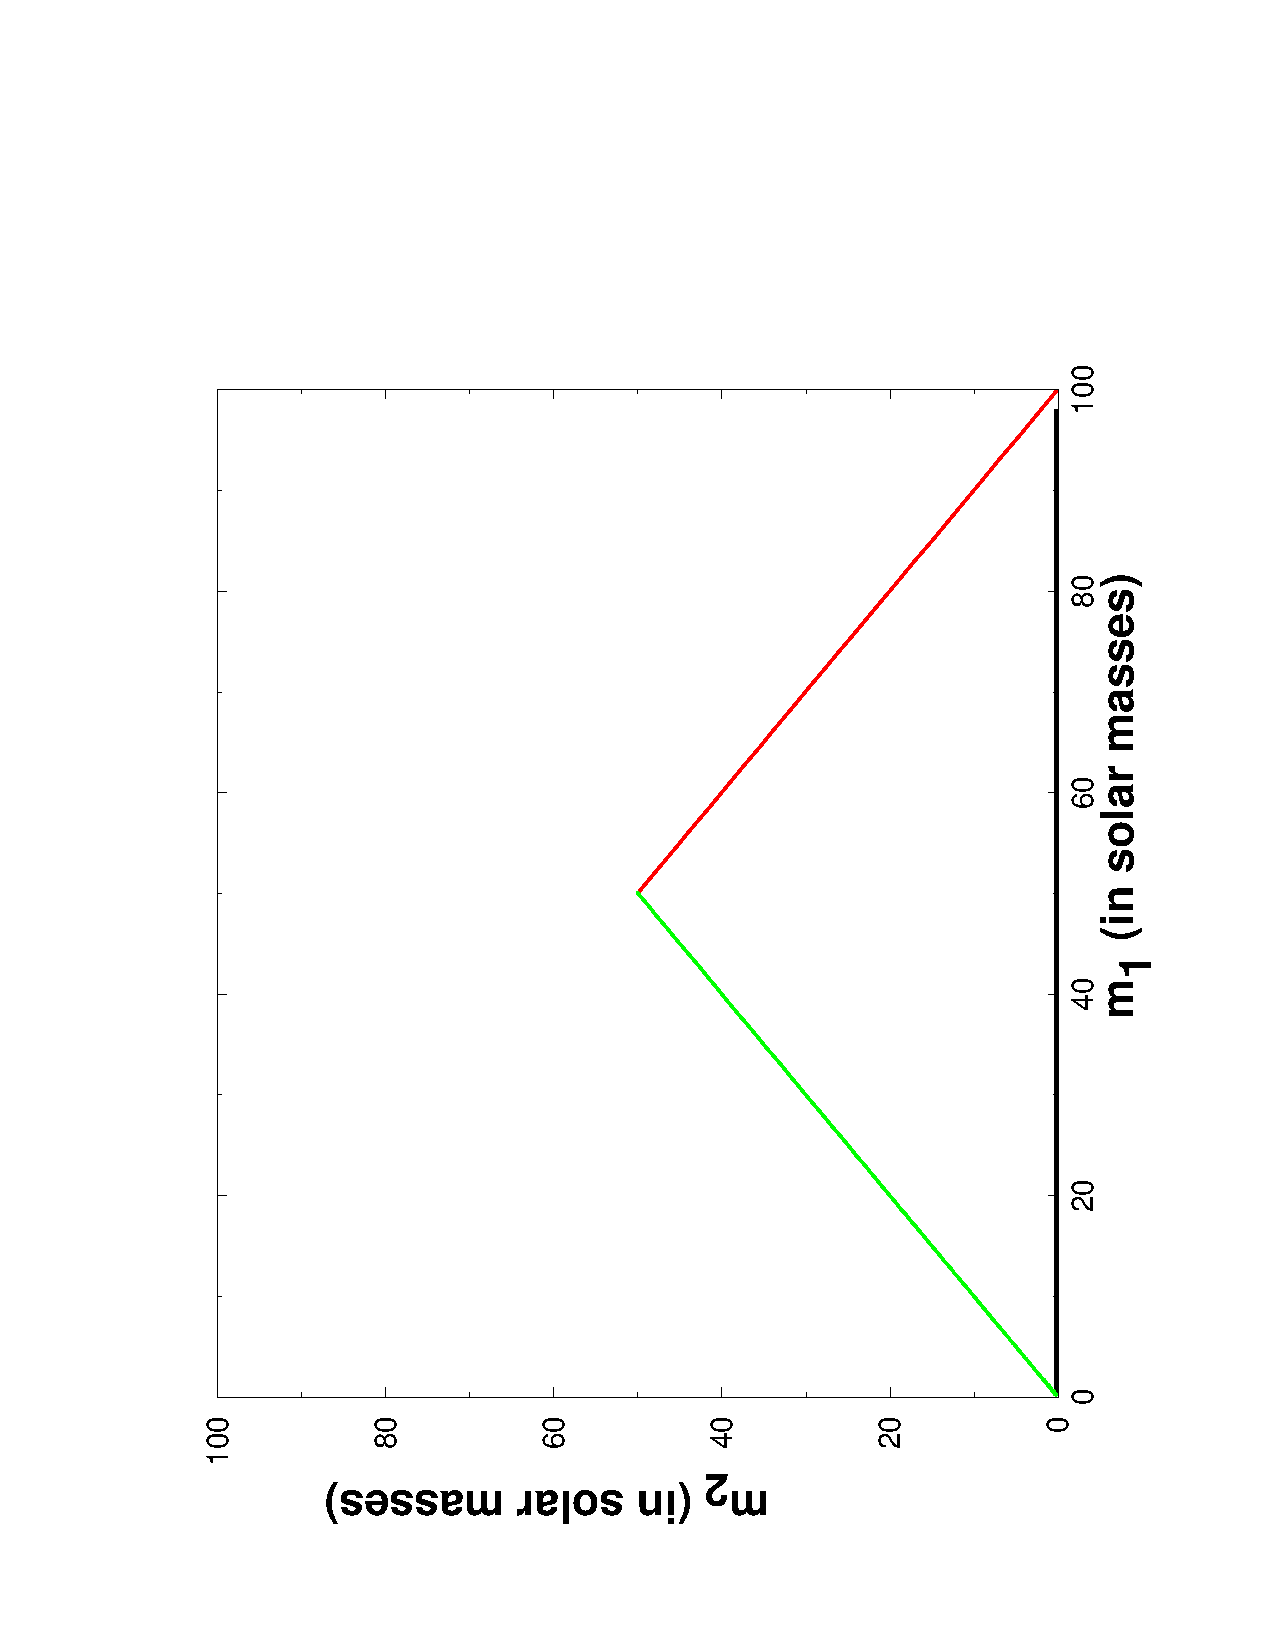
\includegraphics[angle=-90,width=0.49\linewidth]{./LALInspiralBankHm1m2}
\noindent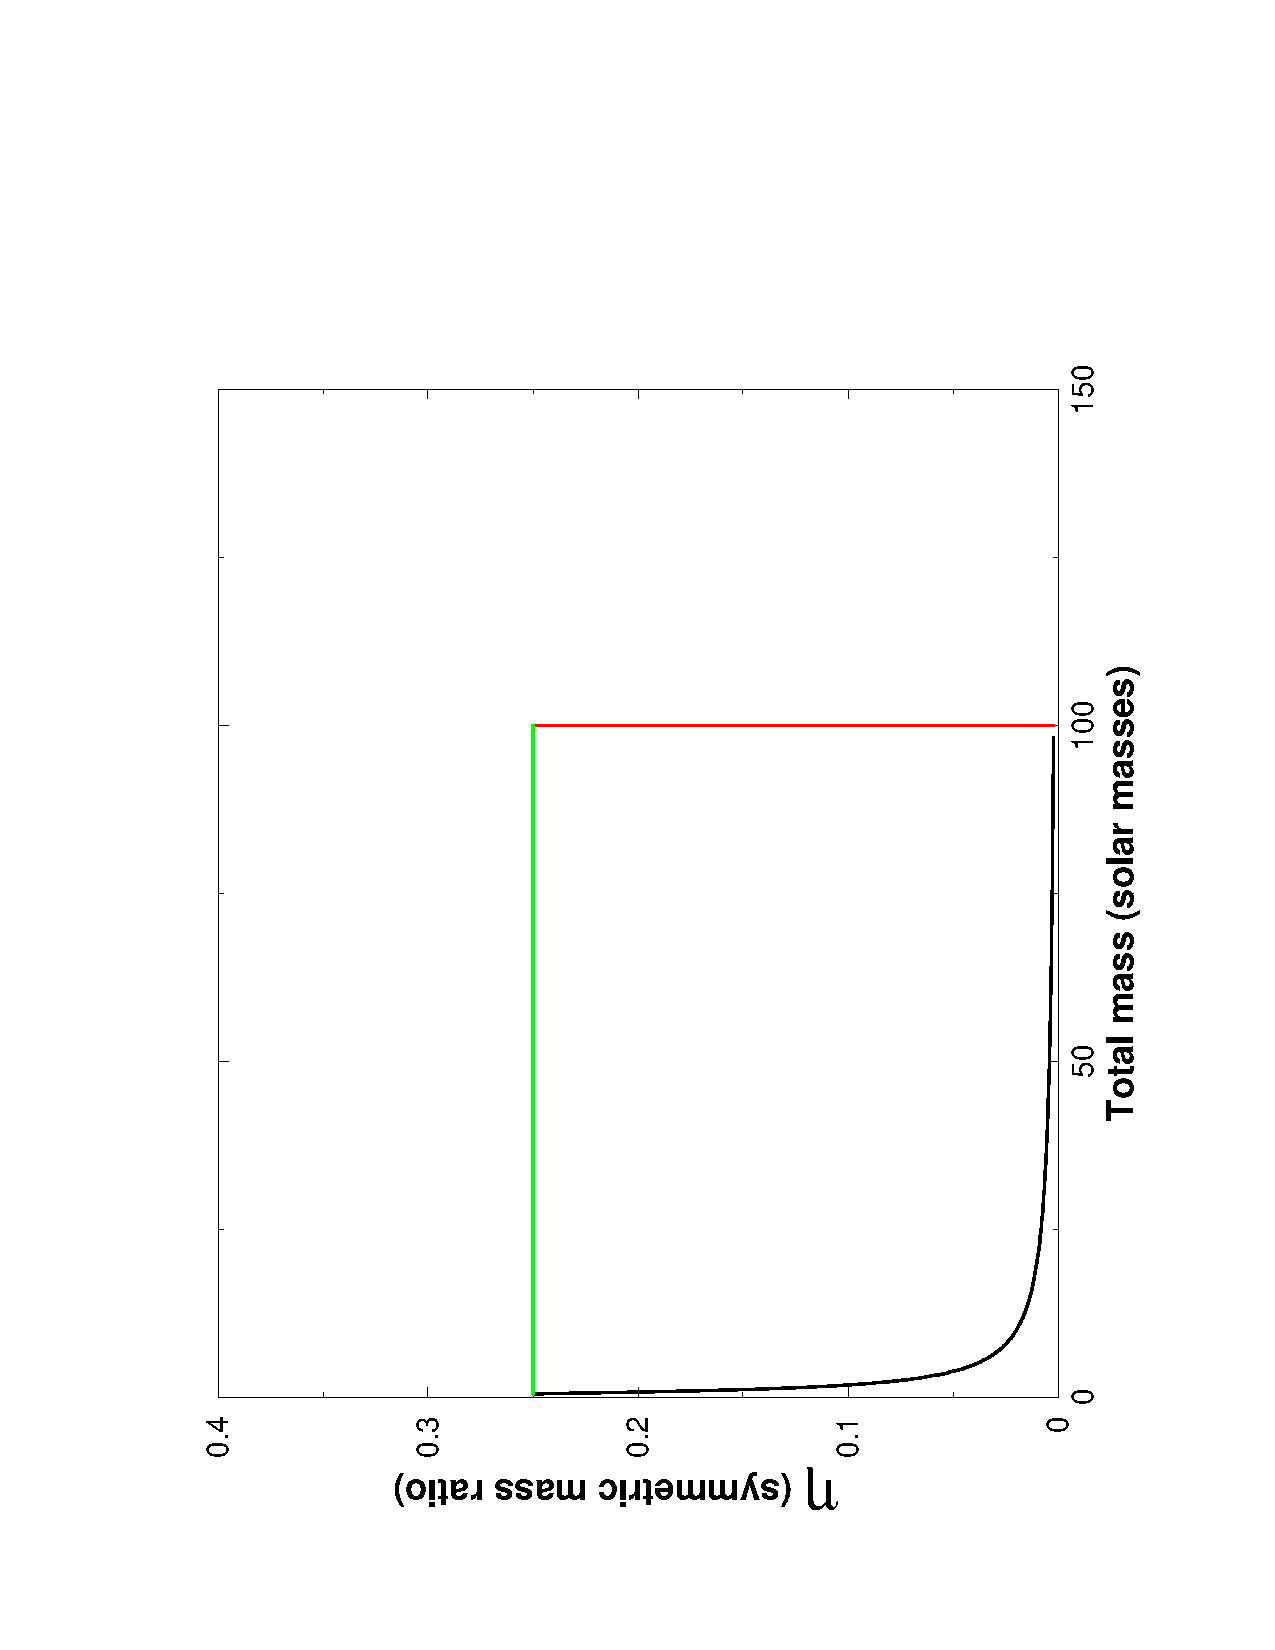
\includegraphics[angle=-90,width=0.49\linewidth]{./LALInspiralBankHtotalMassEta}
\noindent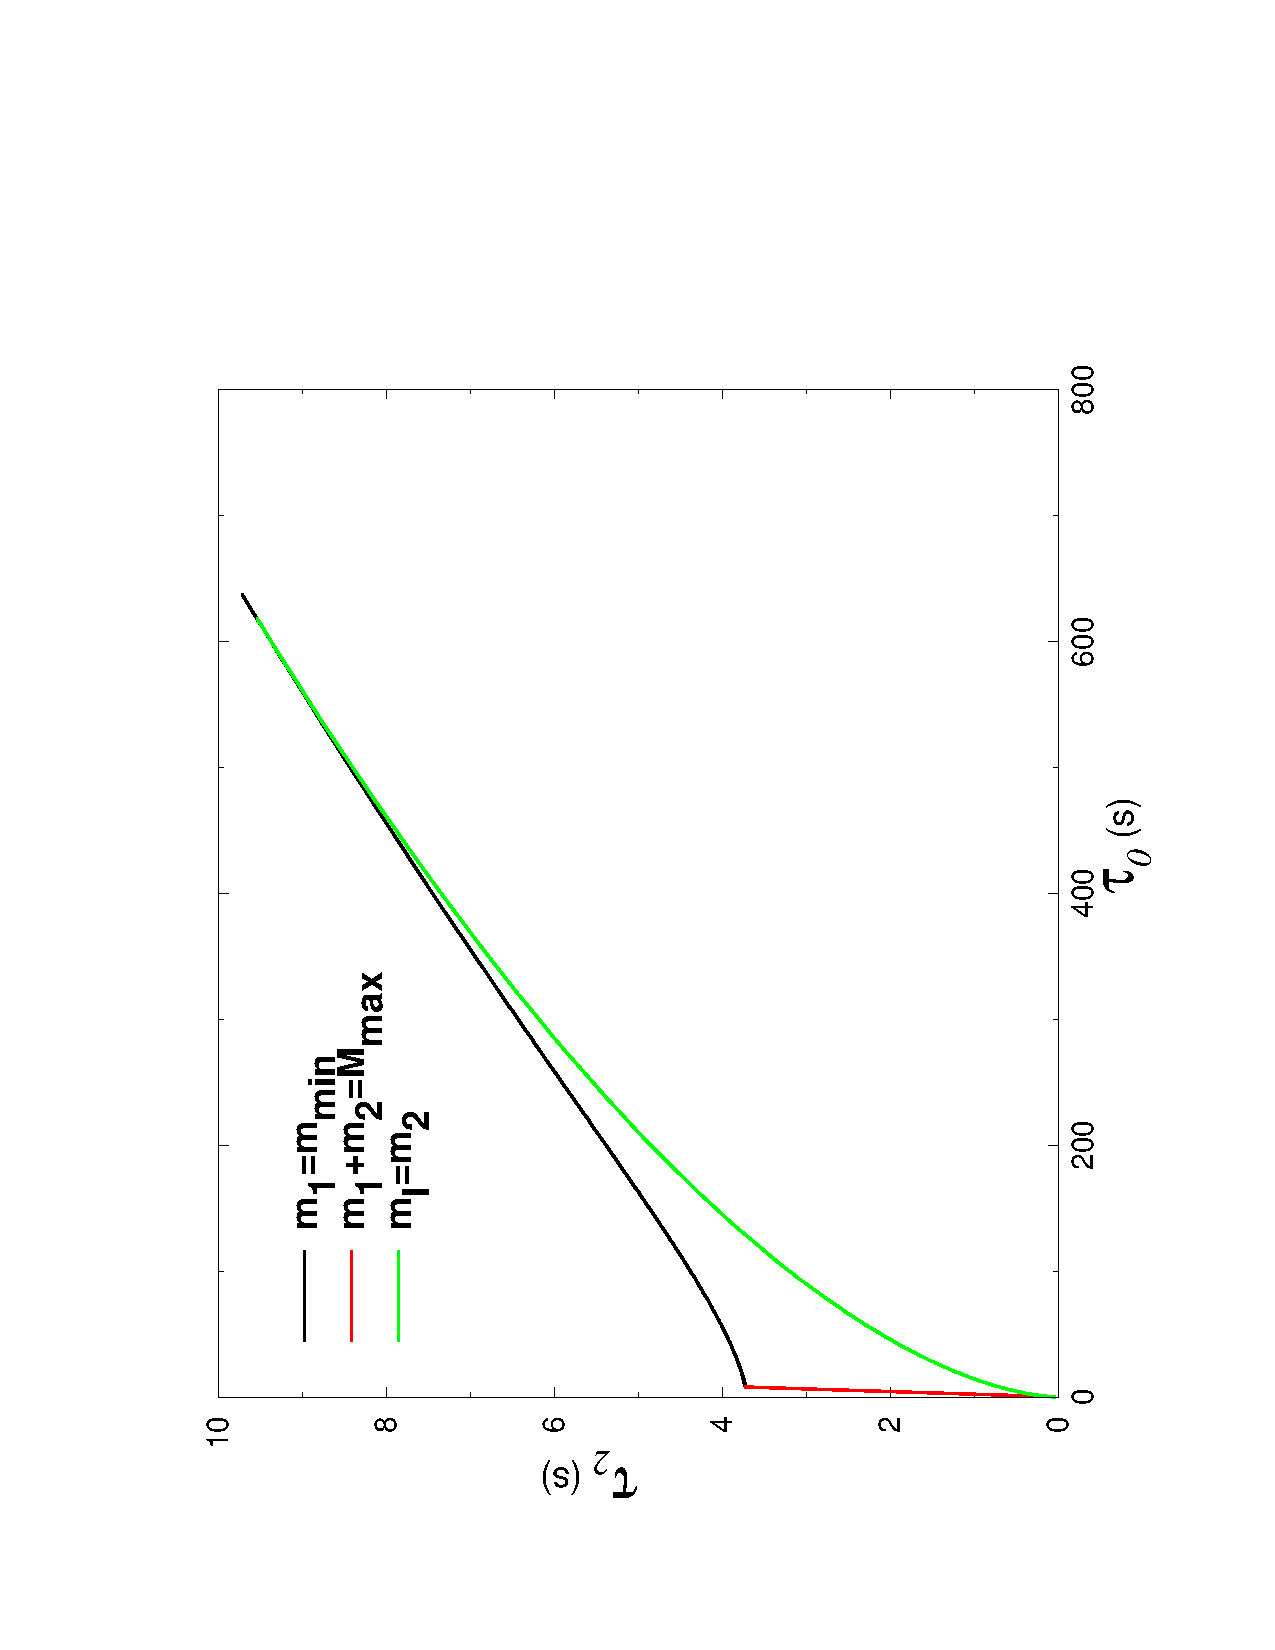
\includegraphics[angle=-90,width=0.49\linewidth]{./LALInspiralBankHt0t2}
\noindent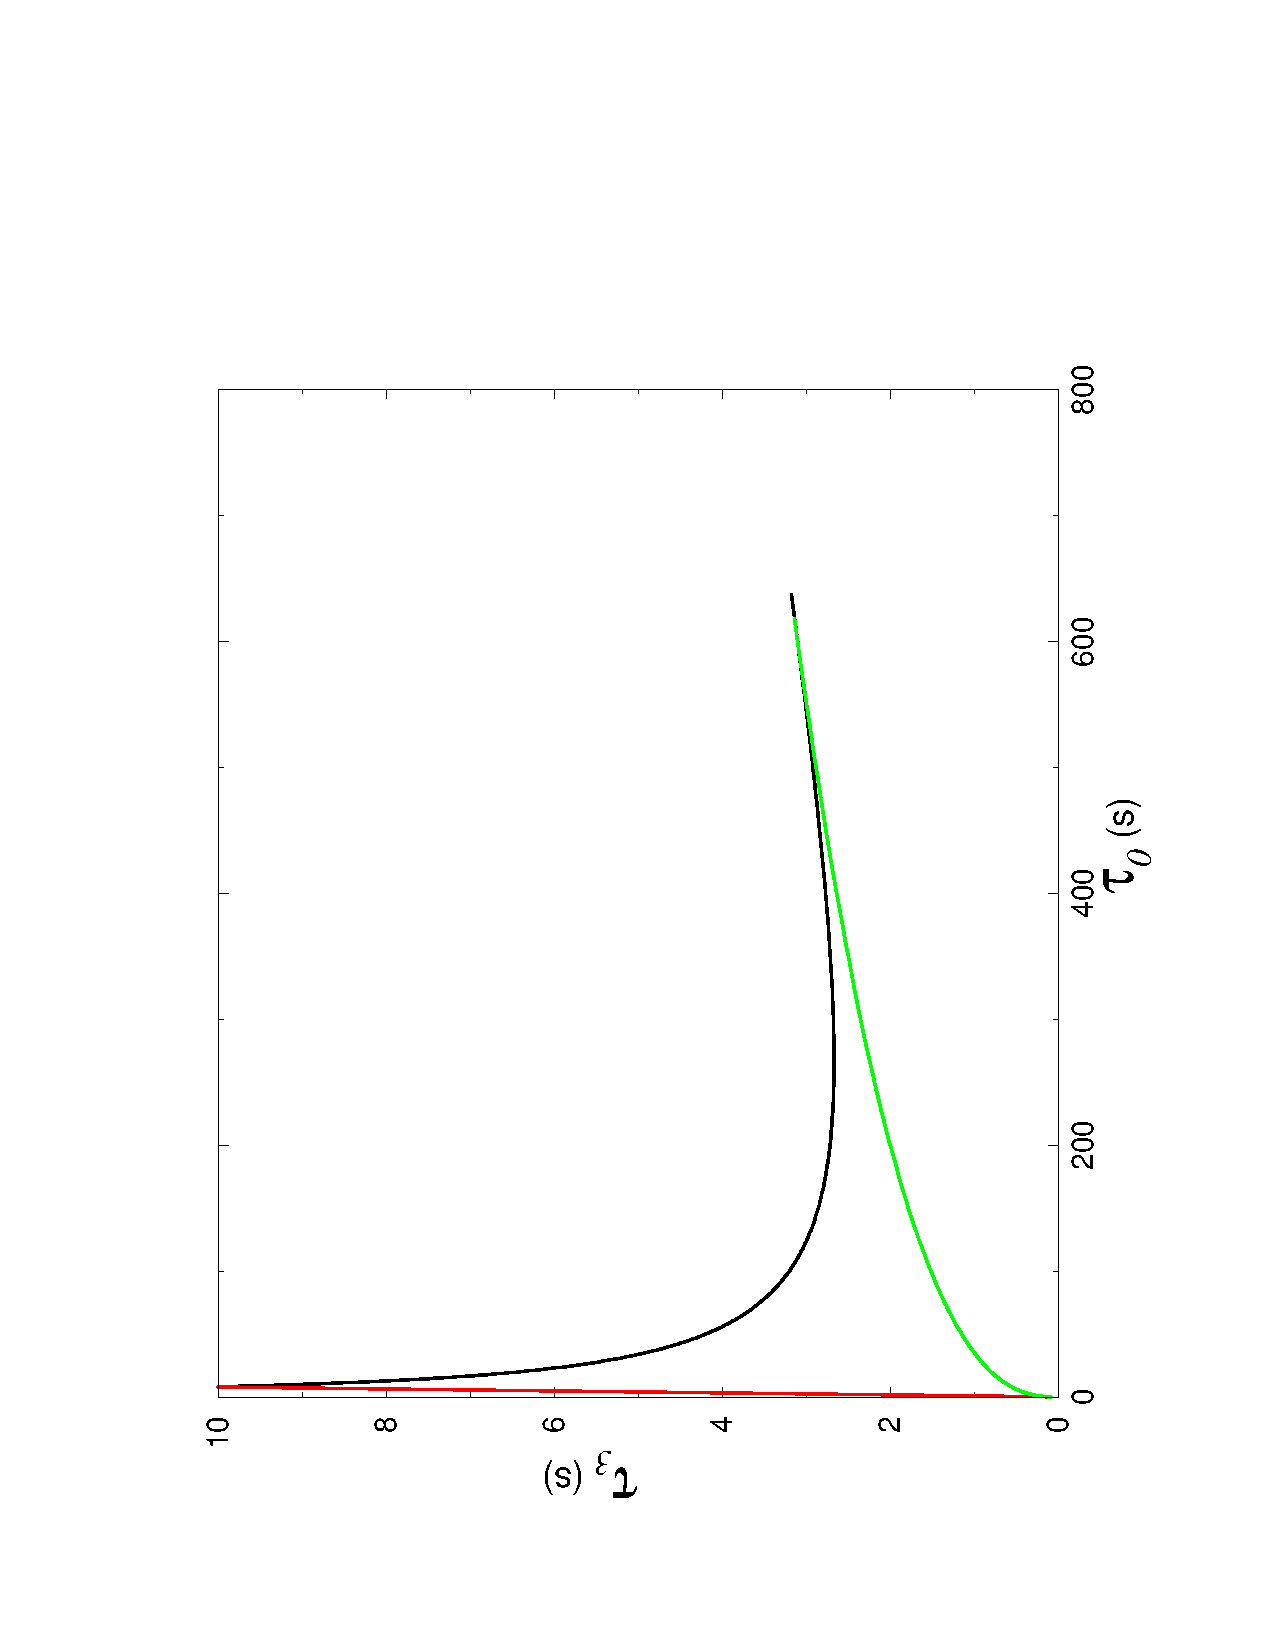
\includegraphics[angle=-90,width=0.49\linewidth]{./LALInspiralBankHt0t3}
}
\caption{The parameter space binary masses and corresponding
chirp-times. Chirp times are computed using an $f_0$ of 40 Hz. Note
that our parameter is specified by $m_1, m_2 >m_{\rm min}$ and
$M=m_1+m_2 < M_{\rm max}$ rather than by $m_{\rm min} < m_1,m_2 < m_{\rm max}.$
(We use capital $M$ to denote the total mass and lower-case $m$ to denote
the component masses.) In the above example $m_{\rm min} = 0.2 M_\odot$
and $M_{\rm max} = 100 M_\odot.$}
\label{fig:chirp-times}
\end{figure}

The number of chirp
times that one can define is determined by the post-Newtonian order
one is working with. At the second post-Newtonian order (i.e.
an approximation accurate to order\footnote{We use units in
which $c=G=1;$ thus $1M_\odot=4.92549095 \times 10^{-6}$~s.} $v^4$) and for
a binary consisting of two non-spinning compact objects in a quasi-circular
orbit, there are
four chirp-times $\tau_k,$ $k=0,\ 2,\ 3,\ 4,$ of which we can choose
any two to characterize the binary:
\begin{equation}
\tau_{0} = \frac{5M}{256 \eta v_{0}^{8}}
\end{equation}
\begin{equation}
\tau_{2} = \frac{5M}{192 \eta v_{0}^{6}} \left( \frac{743}{336} + \frac{11}{4} \eta \right)
\end{equation}
\begin{equation}
\tau_{3} = \frac{\pi M}{8 \eta v_{0}^{5}}
\end{equation}
\begin{equation}
\tau_{4} = \frac{5M}{128 \eta v_{0}^4} \left( \frac{3\,058\,673}{1\,016\,064} + \frac{5429}{1008}
\eta +
\frac{617}{144} \eta^{2} \right)
\end{equation}
where $m$ is the total mass of the
binary, $\eta=m_1m_2/m^2$ is the symmetric mass ratio and
$v_0 = (\pi m f_0)^{1/3}$ is a fiducial velocity parameter corresponding
to a fiducial frequency $f_0,$ usually chosen to be the {\it lower
frequency cutoff} of the detector sensitivity.

This algorithm allows one to choose
a coarse grid of templates either in the $\tau_0$-$\tau_2$
or $\tau_0$-$\tau_3$ space depending on the value of the
\texttt {enum}
\texttt {CoordinateSpace,} which can take one of two values:
\texttt {Tau0Tau2} or \texttt {Tau0Tau3.} The shape of the coordinate
spaces for some interesting range of masses is shown
in Fig.~\ref{fig:chirp-times}. The important point to note in these
figures is that the $\eta=1/4$ curve spans from the {\it minimum} to the
{\it maximum} value of the {\it Newtonian chirp-time} $\tau_0.$  This
feature will be used in the construction of the grid. Note that
the minimum (maximum) value of the Newtonian chirp-time occurs when
the two masses are equal and the total mass is a maximum (minimum).

\subsection{Coarse Grid Algorithm : the square placement}

The coarse grid algorithm used in this module is most economically
described by the following main steps in the algorithm:
\begin{enumerate}
\item Compute the minimum and maximum chirp-times corresponding to the
search space: $(\tau_0^{\rm min}, \tau_0^{\rm max}),$
$(\tau_3^{\rm min}, \tau_3^{\rm max})$ (or\footnote{In what follows
we will only mention $\tau_3$; however, the algorithm is itself valid,
and has been implemented, in the case of $(\tau_0,\tau_2)$ too.}
$(\tau_2^{\rm min}, \tau_2^{\rm max})$)

 \item Choose a lattice of templates along the equal mass curve.

\item Lay a rectangular grid in the rectangular region defined by
the minimum and maximum values of the chirp-times and retain only
if (a) the point lies in the parameter space, OR (b) one of the
vertices defined by the rectangle lies in the parameter space.
If, instead of choosing the templates as specified in (b), we accept
every template whose span has a non-zero overlap with the parameter
space, then we
would generate too many spurious templates, especially in the low-mass
region. This is because of the following reason:
We have chosen to lay templates along the
equal-mass curve and the parameter space is very thin for large values
of $\tau_0$ along this curve -- the region where the `distance'
between the $m_1=m_{\rm min}$ curve and the equal-mass curve is
smaller than one minimal-match.
By laying templates in a rectangular grid in the
$\tau_0$-$\tau_3$ space we would be encoutering templates in this
region and just above the equal-mass curve
none of whose vertices would be within the search space. By
throwing away such templates there is no danger of creating any
`holes' in the parameter space. Indeed, criterion (b)
will help in filling the holes below the $m_1=m_{\rm min}$
curve that would be created by accepting templates that meet
only criterion (a).

\end{enumerate}

The algorithm begins by identifying the vertices at the boundary of
the search space corresponding to the range of masses over which one
intends to carry out a search. It first chooses a set of templates
along the equal mass curve and then lays a rectangular lattice
of templates in the rectangular region defined by
$(\tau_0^{\rm min}, \tau_3^{\rm min}),$ $(\tau_0^{\rm max}, \tau_3^{\rm min}),$
$(\tau_0^{\rm max}, \tau_3^{\rm max}),$ and $(\tau_0^{\rm min}, \tau_3^{\rm max}).$

\subsubsection{Parameters specifying a coarse grid}

The algorithm takes as input the structure
\texttt {InspiralCoarseBankIn} and returns a pointer to an array of
type \texttt{InspiralTemplateList} and the number of elements in the
array.  \texttt{InspiralCoarseBankIn} is designed to provide the coarse
bank algorithm with information about the search space such as the
minimum mass of component stars, maximum total mass, etc., as well as
other parameters not directly used by the coarse grid algorithm but
are needed by inspiral wave generation algorithms. This is so that
the coarse grid algorithm can correctly set the members of the
\texttt{InspiralTemplateList} structure. In particular, the members
of the \texttt{InspiralCoarseBankIn} structure used by the coarse grid
algorithm are:
\begin{itemize}
\item \texttt {REAL8 mMin,} minimum mass of the component stars
\item \texttt {REAL8 MMax,} maximum total mass of the binary
\item \texttt {REAL8 mmCoarse,} coarse grid minimum match
\item \texttt {REAL8 fLower,} lower frequency cutoff to be used in the computation of the
noise moments
\item \texttt {REAL8 fUpper,} upper frequency cutoff to be used in the computation of the
noise moments
\item \texttt {void (*NoisePsd)(LALStatus *status, REAL8 *shf, REAL8 f),} pointer to
a function that returns the noise spectral density (in units of per Hz$^{-1}$);
\texttt{noisemodels} modules have built in noise power spectral densities
\texttt{LALGEOPsd, LALLIGOIPsd, LALTAMAPsd} and \texttt{LALVIRGOPsd}.
\item \texttt {REAL8 order,} the post-Newtonian order to be used
for wave generation the choices being
\texttt {newtonian, onePN, onePointFivePN, twoPN, twoPointFivePN,
threePN, threePointFivePN}.
\item \texttt {CoordinateSpace space,} the coordinate space in which templates
are laid (the choices being \texttt {Tau0Tau2, Tau0Tau3}; at \texttt{onePN}
order the only choice is \texttt{Tau0Tau2}).
\item \texttt {etamin,} minimum value of eta; must be pre-computed using the
formula \texttt{etamin = mMin * (MMax - mMin) / pow(MMax,2)}
before calling the \texttt {LALInspiralCreateCoarseBank.}
\end{itemize}
Additionally, the user may specify the fine bank minimal match
\texttt{mmFine,} if \texttt{LALInspiralCreateFineBank} is called.
A fine bank can be created only around grid points where the
metric is known.

Other members of the \texttt{InspiralCoarseBankIn} structure that
are not directly used by the coarse grid algorithm but are needed to
correctly set all the members of the \texttt{InspiralTemplate} are:

\begin{itemize}
\item \texttt {REAL8 tSampling,} time-domain sampling rate in Hz.
\item \texttt {REAL8 approximant,} the approximation method to be used
for wave generation which can be anyone of \texttt{TaylorT1, TalorT2,
TaylorT3, TaylorF1, TaylorF2, {\rm or} PadeT1, PadeF1, EOB}. Note that
the placement algorithm is guaranteed to work with only \texttt {TaylorF2}
approximants. A detailed study of approximants that are well captured by
this template placement algorithm is described elsewhere \cite{Sathyaprakash
2001a}.
\item \texttt {GridSpacing,} specify the type of placement to be used. For the
physical template families placement, it must be \texttt{SquareNotOriented,
Hexagonal, HybridHexagonal}. For the non-BCV case, it could be Square,
\texttt{SquarenotOriented, Hexagonal, HexagonalNonOriented}. Concerning
the physical case, the non oriented square placement, as described in this
section, places the template on a square lattice but does not take into
account the orientation of the ellipse, which might cause problem in some
particular cases. The Hexagonal placement was then implemented taking  into
account the orientation of the ellipse. No square placement with the correct
orientation has been implemented since the hexagonal is now used for in the
LIGO analysis. Concerning the non-spinning BCV placement, all 4 cases are
available. However, only the non oriented square placement and oriented
hexagonal placement hav ebeen thouroughly tested as well.

\end{itemize}

\subsection{Coarse Grid Algorithm : the hexagonal placement}
This module has the ability to place the templates on an hexagonal lattice.
This placement reduces by 30\% (as expected) the number of templates used by
the square lattice. Although the algorithm is different (and described in this
documentation), it is based on the same structure and uses the same function
to be called, namely \texttt{LALInspiralCreateCoarseBank}. The lattice is
specified by the variable \texttt{gridSpacing} from the structure \texttt{InspiralCoarseBankIn}, where
the user must set gridSpacing to \texttt{Hexagonal}.

\subsection{Coarse Grid Algorithm : the hybrid hexagonal placement}
A very similar placement place the template on an hexagonal lattice similarly
to the previous hexagonal placement bu has a slightly different placement when
upper an lower boundaries of the parameter space are coverred by a single
template. In such a case, the hexagonal placement is replace by a placement
along the bissectrice of the upper and lower boundaries. See the documentation
for more details. This algorithm is called by setting gridSpacing to  \texttt{HybridHexagonal}.

\subsection{Coarse Grid algorithm: non physical placement (BCV)}
There is also the ability to create a bank for the non-spinning BCV templates.
See the documentation. If so, the user must set approximant to BCV instead of
one of the physical approximant (EOB, TaylorT1, ...).

\newpage\input{LALInspiralBankH}

\begin{thebibliography}{}
\bibitem {Sathyaprakash and Dhurandhar 1991} B.S. Sathyaprakash and
S.V. Dhurandhar, Phys. Rev. D {\bf 44,} 3819 (1991).
\bibitem {Sathyaprakash 1994} B.S. Sathyaprakash, Phys. Rev. D {\bf 50,} R7111
(1994).
\bibitem {OwenAndSathyaprakash:99} B.J. Owen and B.S. Sathyaprakash,
Phys. Rev. D {\bf 60,} 022002 (1999)

\bibitem {Sathyaprakash 2001a} B.S. Sathyaprakash, {\it Effectualness of
template placement algorithtms in capturing different post-Newtonian
inspiral signals} (in preparation).

\bibitem {Owen:96} B.J. Owen, Phys. Rev. D 53, 6749 (1996).
\end{thebibliography}
